\documentclass{article}
\topmargin -0.5in \oddsidemargin -0.25in \textheight 9in
\textwidth 6.5in
\usepackage{graphics}
\usepackage{graphicx}
\usepackage{forest}
\usepackage{tikz}
\usepackage{amsmath}
\usepackage{amssymb}


\newcommand{\shrink}[1]{}

\begin{document}
{\bf ICS 271}

{\bf Fall 2016}

{\bf Student ID : 26642334}

{\bf Student Name: Yu Guo}

{\bf Instructor : Kalev Kask}

{\bf Homework Assignment 3}

{\bf Due Tuesday, 10/25}




\begin{enumerate}

% 1.
\item

  \begin{enumerate}
    \item $<3^9$

    \item - Depth of the tree = 9 (excluding root node)

    - Does the complete game tree contain all the board positions you counted in (a)? 

    ~ No. For example, `less $\bigcirc$ than $\times$' will not appear in the tree. 

    - Does it contain additional board positions? 

    ~ No.

    \item See Figure 1. 

    \item See Figure 1.

    \item See Figures 2-4.


  \end{enumerate}


% 2.
\item

Yes. The game tree is complete, so alpha-beta pruning algorithm is guaranteed to force a win.

% 3.
\item
  
  \begin{enumerate}
    \item First node from left to right. (See Figure 5)

    \item See Figure 5.
  \end{enumerate}


% 4.
\item

To prove this theory, the key idea is to prove that after each min, max and chance node, the choice would not be changed. 
Suppose that the value of each child node are $x_1,x_2,\dots,x_n$, and transformation is $5ax+b$, where $a>0$. We have

$$\min(5ax_1+b,5ax_2+b,\dots,5ax_n+b) = 5a\min(x_1,x_2,\dots,x_n)+b$$
$$\max(5ax_1+b,5ax_2+b,\dots,5ax_n+b) = 5a\max(x_1,x_2,\dots,x_n)+b$$
$$p_1(ax_1+b)+p_2(ax_2+b)+\dots+p_n(ax_n+b) = a(p_1x_1+p_2x_2+\dots+p_nx_n)+b$$

Since $x>y \Rightarrow ax+b>ay+b$ if $a>0$, that means the linear transformation ($a>0$) of child nodes would not affect the choice of parent node. Maximum or minimum choice would not be changed. 
The best choice at the root will be the same as the best choice in the original tree.

% 5.
\item

Take the average over all $n$ executions is Monte Carlo method. According to \textbf{Strong Law of Large Numbers},
$$\frac{1}{n}\sum_{i=1}^n x_i \xrightarrow[]{n\rightarrow\infty} \mathbf{E}(\mathbf{X}), x_i\in\mathbf{X}$$
The average of more samples leed to the true expected value.
Mathematically, we can never get correct results, but in practice, with a large number of $n$, it's a very good estimation of 
the real value.

\end{enumerate}


    \begin{figure}[ht]
    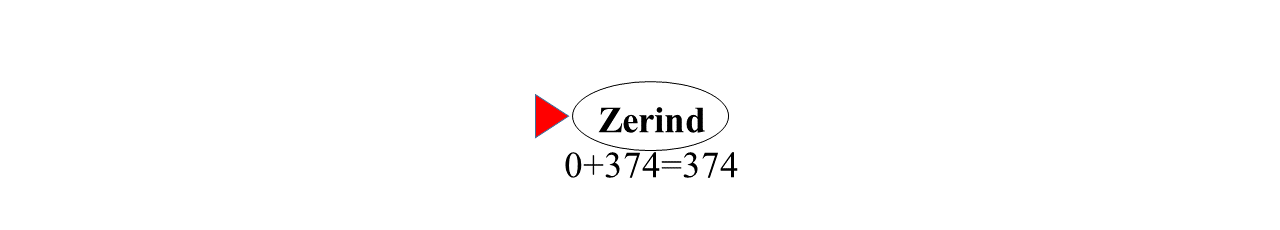
\includegraphics[width=\textwidth]{figure/Slide1.PNG}
    \caption{}
    \end{figure}
    \begin{figure}[ht]
    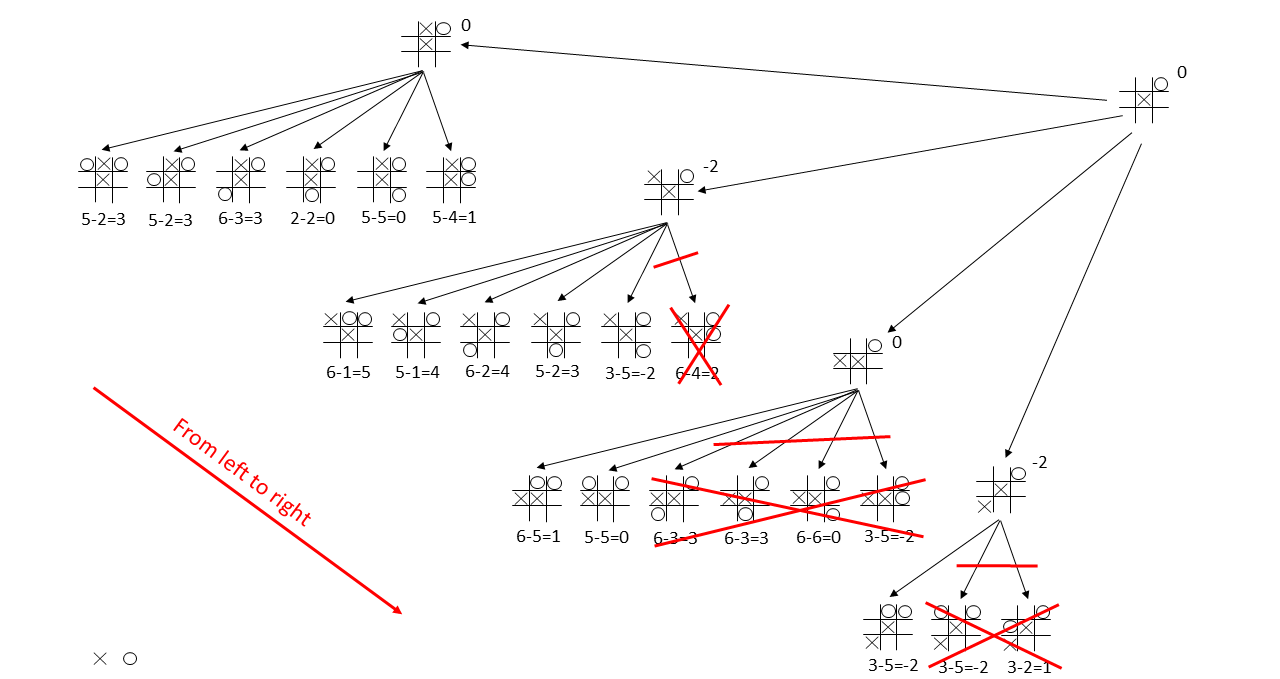
\includegraphics[width=\textwidth]{figure/Slide2.PNG}
    \caption{}
    \end{figure}
    \begin{figure}[ht]
    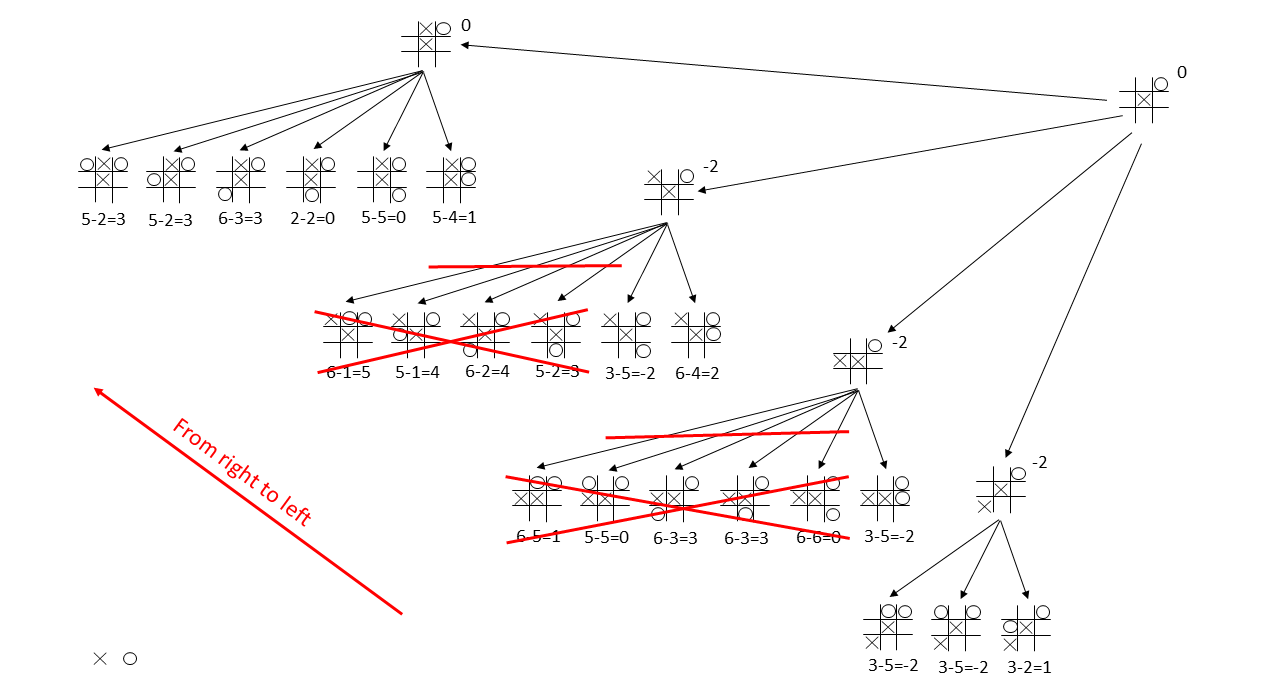
\includegraphics[width=\textwidth]{figure/Slide3.PNG}
    \caption{}
    \end{figure}
    \begin{figure}[ht]
    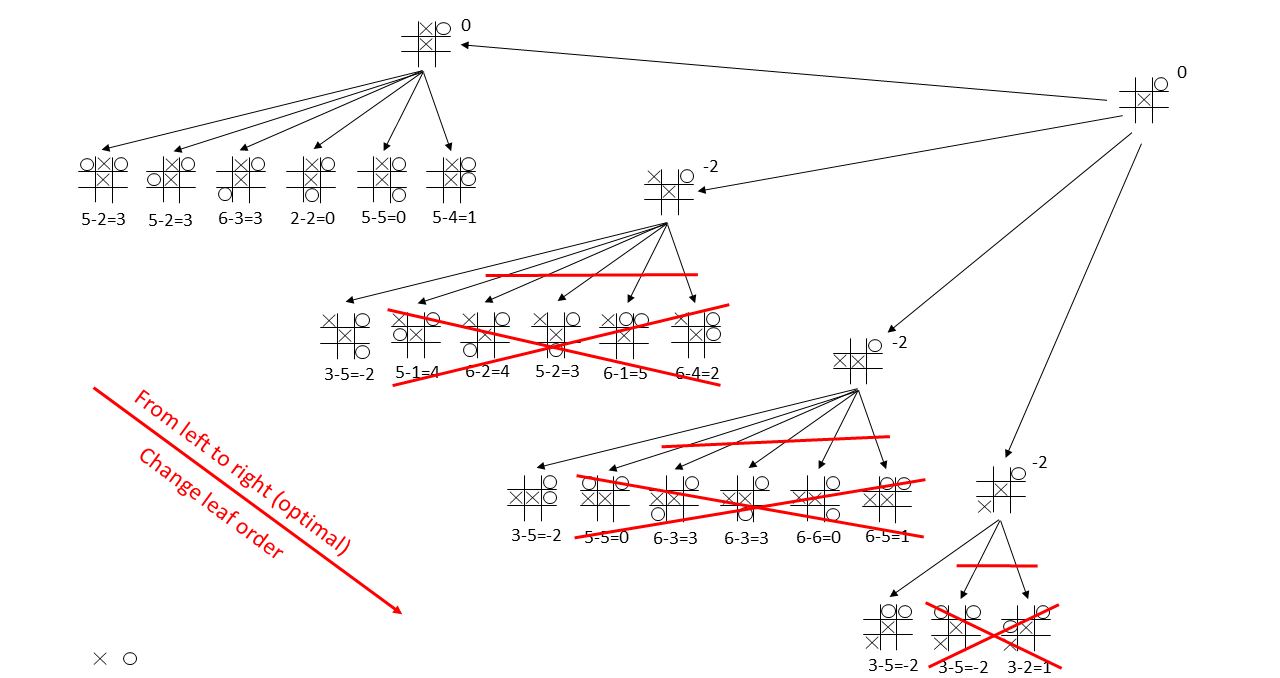
\includegraphics[width=\textwidth]{figure/Slide4.PNG}
    \caption{}
    \end{figure}
    \begin{figure}[ht]
    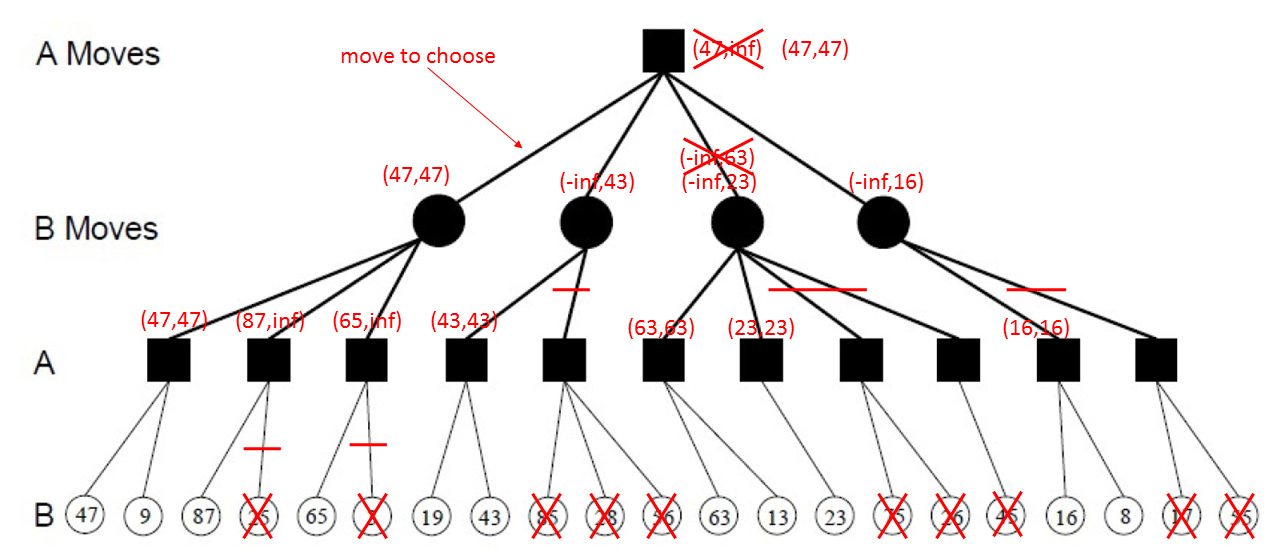
\includegraphics[width=\textwidth]{figure/Slide5.PNG}
    \caption{}
    \end{figure}

\end{document}